\def\numprint#1.{#1{,}}
\def\stackon#1#2{\begin{array}{@{}c@{}}#2\\[-2pt]#1
                 \end{array}}
                 
	\spis{Papierem na księżyc}
{Grzegorz Szymanek} 
                 
	\wtyt{Papierem na księżyc}
	\waut{Grzegorz SZYMANEK*} 
	\aafil{Student, Wydział Fizyki, Uniwersytet Warszawski}
	
	

	Znanym faktem jest, że zginając kartkę wpół, dokonujemy jej dwukrotnego pogrubienia.
	Z~każdym zgięciem następne jest coraz trudniejsze -- aż do 
	momentu, w~którym dokonanie jeszcze jednego jest już niemożliwe. 
	Nasuwa się więc nieuchronne pytanie: ile właściwie razy można zgiąć daną kartkę wpół?
	Tę właśnie liczbę spróbujemy wyznaczyć, przyjmując, że kartkę zginać będziemy naprzemiennie
	po długości i~szerokości.
	Niech $n$ oznacza liczbę dokonanych zgięć; $\mathcal{L}_n$, $\mathcal{W}_n$, $\mathcal{D}_n$ -- 
	odpowiednio: długość, szerokość i~grubość kartki po $n$ zgięciach. 
	Na początek zdefiniujmy założenia, na których będziemy bazować 
	podczas dalszego zgłębiania pomysłu:	
		\marg{ 
                  \begin{tikzpicture}
\node at(1.55,0){
\includegraphics[scale=.46]{papier01.png}};
\draw [decorate,decoration = {brace,raise=4pt}] (-.4,-.6) --  (-.4,0)node[pos=.5,left=5pt]{$2d$};
 \draw [decorate,decoration = {brace,mirror,raise=6pt}] (-.38,-.6) --  (-.09,-.6)node[pos=.5,below=8pt]{$d$};
 \draw [decorate,decoration = {brace,mirror,raise=6pt}] (-.09,-.6) --  (2.65,-.6)node[pos=.5,below=8pt]{$l_{1}$};
 \draw [decorate,decoration = {brace,mirror,raise=6pt}] (2.65,-.6) --  (3.48,.01)node[pos=.5,below=7pt,xshift=8pt]{$w_{0}$};
\end{tikzpicture}\\[4pt]
		\text{Rys. 1}. Pierwsze zagięcie -- wykonane równolegle do krawędzi szerokości\bigskip

                  \begin{tikzpicture}
\node at(1.3,.3){
\includegraphics[scale=.46]{papier03.png}};
\draw [decorate,decoration = {brace,raise=4pt}] (-.4,-.6) --  (-.4,.6)node[pos=.5,left=5pt]{$4d$};
 \draw [decorate,decoration = {brace,mirror,raise=6pt}] (-.38,-.6) --  (-.09,-.6)node[pos=.5,below=8pt]{$d$};
 \draw [decorate,decoration = {brace,mirror,raise=6pt}] (-.09,-.6) --  (1.73,-.6)node[pos=.5,below=8pt]{$l_{1}$};
 \draw [decorate,decoration = {brace,mirror,raise=6pt}] (1.7,-.6) --  (2.48,.01)node[pos=.5,below=7pt,xshift=8pt]{$w_{1}$};
 \draw [decorate,decoration = {brace,mirror,raise=6pt}]  (2.48,.01) -- (2.8,.3)node[pos=.5,below=7pt,xshift=8pt]{$2d$};
\end{tikzpicture}\\[4pt]
                \text{Rys. 2}. Drugie zagięcie -- wykonane równolegle do krawędzi długości
                \bigskip
                
 \begin{tikzpicture}
\node at(1.63,.91){
\includegraphics[scale=.46]{papier02.png}};
\draw [decorate,decoration = {brace,raise=4pt}] (-.4,-.6) --  (-.4,1.84)node[pos=.5,left=5pt]{$8d$};
 \draw [decorate,decoration = {brace,mirror,raise=6pt}] (-.38,-.6) --  (1.7,-.6)node[pos=.5,below=8pt]{$l_{2}$};
 \draw [decorate,decoration = {brace,mirror,raise=6pt}] (1.7,-.6) --  (2.92,-.6)node[pos=.5,below=7pt]{$4d$};
\end{tikzpicture}\\[4pt]
		\text{Rys. 3}. Trzecie zagięcie -- wykonane równolegle do krawędzi szerokości
	}
	
	 \begin{enumerate}
		\item Złożenie kartki wpół oznacza, że na ,,zewnątrz'' zagięcia 
		powstaje łuk kolisty o~takiej długości, by suma ,,zewnętrznej'' 
		powierzchni odpowiadała powierzchni kartki przed złożeniem.
		\item ,,Wewnętrzna'' część zagięcia jest punktowa -- kartka zostaje w~tym miejscu ,,złamana''.  
		\item Konsekwencją punktów 2 i~3 jest fakt, że objętość kartki 
		na obszarze zagięcia maleje dwukrotnie. Przyjąć więc można jedną 
		z~dwóch możliwych interpretacji:
		\begin{itemize}
			\item średnia gęstość kartki na zagięciu jest dwukrotnie 
			większa niż przed wykonaniem zgięcia,
			\item po wykonaniu zagięcia po stronie przeciwnej niż 
			nowo utworzony łuk powstaje klin ,,kompensujący'' ubytek 
			w~objętości.\vspace*{1pt}
		\end{itemize}
		Niezależnie od tego, którą z~powyższych opcji przyjmiemy, 
		warunki 1 i~2 pozostają spełnione.
	\end{enumerate}
	
        \ptyt{Tym samym możemy rozpocząć naszą przygodę% ze składaniem
          .}
	W~celu ułatwienia obliczeń wprowadźmy oznaczenia 
	(jak na rysunkach): $l_m$~--~długość płaszczyzny kartki (bez łuku), 
	$w_u$ -- adekwatnie, szerokość płaszczyzny, $d$~--~początkowa grubość kartki, 
	gdzie $m$ oraz $u$ należą do zbioru $ \{0,1,2,\dots\}$.\\
	W~pierwszej kolejności wyraźmy grubość kartki po $n$ zgięciach:
	\begin{gather*}
		\mathcal{D}_n = d\cdot 2^{n}.
	\end{gather*}	
	Dalej przyjmijmy następującą definicję długości i~szerokości: operację rozpoczynamy 
	od wykonania zagięcia równoległego do krawędzi szerokości $\mathcal{W}$,
	następnie do krawędzi długości $\mathcal{L}$, znowu $\mathcal{W}$ itd.
	Długość i~szerokość wybieramy więc, określając kolejność wykonywanych zgięć
	($l_0$ sprzecznie z~lingwistyczną konwencją nie musi być większe od $w_0$).
	\begin{szeroko}
	
	\begin{tcolorbox}[lower separated=false, colback=white, colframe=magenta,fonttitle=\bfseries, colbacktitle=black, coltitle=white]
          \begin{enumerate}[label={$n=\arabic*$},itemsep=6pt]%,leftmargin=20pt
            			\begin{multicols}{3}
				% make text smaller in itemize
				%\footnotesize
				\item   $\begin{gathered}[t]
					\mathcal{W}_1 = \mathcal{W}_0\\
					2l_1 + \pi d = l_0 + 0\\
					l_1 = \frac{1}{2}(l_0-\pi d)\\
					\mathcal{L}_1 = l_1 + d
				\end{gathered}$
				\item   $\begin{gathered}[t]
					\mathcal{L}_2 = \mathcal{L}_1\\
					2 w_1 + 2\pi d = \mathcal{W}_1 = w_0+0\\
					w_1 = \frac{1}{2}(w_0-\pi\cdot 2d)\\
					\mathcal{W}_2 = w_1 + 2d
				\end{gathered}$
				\item   $\begin{gathered}[t]
					\mathcal{W}_3 = \mathcal{W}_2\\
					2 l_2 + 4\pi d = \mathcal{L}_2 = l_1 + d\\
					l_2 = \frac{1}{2}(l_1 + d - \pi\cdot 4d)\\
					\mathcal{L}_3 = l_2 + 4d
				\end{gathered}$
				\item   $\begin{gathered}[t]
					\mathcal{L}_4 = \mathcal{L}_3\\
					2 w_2 + 8\pi d = \mathcal{W}_3=w_2+ 2d\\
					w_2 = \frac{1}{2}(w_1 + 2d - \pi\cdot 8d)\\
					\mathcal{W}_4 = w_2 + 8d
				\end{gathered}$
				\item   $\begin{gathered}[t]
					\mathcal{W}_5 = \mathcal{W}_4\\
					2 l_3 + 16\pi d = \mathcal{L}_4=l_2 + 4d\\
					l_3 = \frac{1}{2}(l_2 + 4d -\pi\cdot 16d)\\
					\mathcal{L}_5 = l_3 + 16d
				\end{gathered}$
				\item   $\begin{gathered}[t]
					\mathcal{L}_6 = \mathcal{L}_5\\
					2 w_3 + 32\pi d = \mathcal{W}_5=w_4+ 8d\\
					w_3 = \frac{1}{2}(w_2 + 8d - \pi\cdot 32d)\\
					\mathcal{W}_6 = w_3 + 32d
				\end{gathered}$
			\end{multicols}
		\end{enumerate}
	\end{tcolorbox}
      \end{szeroko}
      
	Mając tę postać, można już utworzyć wzór ogólny na $l_m$ (oczywiście dla $m > 0$):
	\begin{gather*}
	l_m = \frac{1}{2}(l_{m-1}+ \lfloor 4^{m-2}\rfloor d - \pi \cdot  4^{m-1} d).
	\end{gather*}
		  Rozwijając powyższą rekurencję (podstawiamy kolejno wzory pod $l_{m-1}$, potem~$l_{m-2}$ itd.), 
		dostajemy sumę, którą można na powrót zwinąć, stosując wzór na sumę ciągu geometrycznego, i~zastępujemy
 tym samym wzór rekurencyjny iteracyjnym:
		\begin{gather*}
			l_m = \frac{1}{2^{m}}l_0 + d\left[\frac{1}{2^{m-1}}\frac{1-8^{m-1}}{1-8}\right] - \pi d{\left[\frac{1}{2^{m}}\frac{1-8^{m}}{1-8}\right]}.
		\end{gather*}
		Wyobraźmy sobie teraz przypadek skrajny, po którego przekroczeniu % (nie zawsze musi wystąpić)
		wykonanie następnego zgięcia będzie niemożliwe (\text{rys. 4}).
		
		
		\marg{ \begin{tikzpicture}
\node at(1.05,1.2){
\includegraphics[scale=.46]{papier2.png}};
\draw [decorate,decoration = {brace,mirror,raise=4pt}] (2.65,-.17) --  (2.65,3)node[pos=.5,right=6pt]{$D_{m}$};
 \draw [decorate,decoration = {brace,mirror,raise=6pt}] (-.38,-.6) --  (1.37,-.6)node[pos=.5,below=8pt]{$D_{m-1}$};
\end{tikzpicture}\\[4pt]
			\text{Rys. 4}. Skrajny przypadek (kartki nie da się już złożyć)}%	
		Widać, że zachodzić musi:
		\begin{gather*}
			l_m \geq 0.
		\end{gather*}
		Z~tego warunku, po krótkich przekształceniach, otrzymujemy nierówność:
		\begin{gather*}
			m \leq  \log_8\left(\frac{\frac{7}{d}l_0 - 2 + \pi}{\pi - \frac{1}{4}}\right).
		\end{gather*}
		Podobne wyprowadzenie przeprowadzamy dla szerokości $w_u$ i~otrzymujemy:		
		\begin{gather*}
			u~\leq \log_8\left(\frac{\frac{7}{2d}w_0 - 2 + \pi}{8\pi - 2}\right) + 1.
		\end{gather*}
		\Magenta{\bf                   Wystarczy teraz określić liczbę zgięć wzdłuż krawędzi $\mathcal{L}$ i $\mathcal{W}$.}
		Ponieważ~liczba zgięć jest liczbą całkowitą oraz zachodzą nierówności 
		postaci $m,u\leq\dots$, mamy:
		\begin{gather*}
			m =  {\left\lfloor\log_8\left(\frac{\frac{7}{d}l_0 - 2 + \pi}{\pi - \frac{1}{4}}\right)\right\rfloor},\\
			u ={ \left\lfloor\log_8\left(\frac{\frac{7}{2d}w_0 - 2 + \pi}{\pi - \frac{1}{4}}\right)\right\rfloor}.
		\end{gather*}
	Powyższe równości określają maksymalną liczbę zgięć kolejno dla krawędzi~$\mathcal{L}$ i~$\mathcal{W}$
        (przy założeniu, że przy zginaniu jednej z~krawędzi było możliwe zgięcie tej drugiej).
        
		Jeśli $m>u$, mamy ciąg zgięć (np. tutaj $m=n+3$):
		\begin{gather*}
			\underbrace{\stackon{\mathcal{L}}{^1} \rightarrow \stackon{\mathcal{W}}{^1} \rightarrow \stackon{\mathcal{L}}{^2} \rightarrow \stackon{\mathcal{W}}{^2} \rightarrow \dots \rightarrow \stackon{\mathcal{W}}{^u} \rightarrow \stackon{\mathcal{L}}{^{m-2}}}_{\mbox{Cały możliwy do wykonania ciąg zgięć}} \rightarrow \stackon{\mathcal{L}}{^{m-1}} \rightarrow \stackon{\mathcal{L}}{^m}.
		\end{gather*}
		Czyli całkowita liczba zgięć dla $m>u$ to $n = 2u + 1$.\\
		Jeśli natomiast $m\leq u$, mamy ciąg zgięć (np. tutaj $m=u-3$):
		\begin{gather*}
			% \underbrace{\mathcal{L}^{1} \rightarrow \mathcal{W}^{1} \rightarrow \mathcal{L}^{2} \rightarrow \mathcal{W}^{2} \rightarrow \dots \rightarrow \mathcal{L}^{m} \rightarrow \mathcal{W}^{u-2}}_{\mbox{Cały możliwy do wykonania ciąg zgięć}} \rightarrow \mathcal{W}^{u-1} \rightarrow \mathcal{W}^{u}
			\underbrace{\stackon{\mathcal{L}}{^1} \rightarrow \stackon{\mathcal{W}}{^1} \rightarrow \stackon{\mathcal{L}}{^2} \rightarrow \stackon{\mathcal{W}}{^2} \rightarrow \dots \rightarrow \stackon{\mathcal{L}}{^m} \rightarrow \stackon{\mathcal{W}}{^{u-2}}}_{\mbox{Cały możliwy do wykonania ciąg zgięć}} \rightarrow \stackon{\mathcal{W}}{^{u-1}} \rightarrow \stackon{\mathcal{W}}{^u}.
		\end{gather*}	
	Czyli całkowita liczba zgięć dla $m\leq u$ to $u = 2m$.
	Ogólny wzór na $n$ ma postać:
	\begin{tcolorbox}[lower separated=false, colback=white, colframe=magenta, fonttitle=\bfseries, colbacktitle=black, coltitle=white]
		$$
			n = \begin{cases}
				2u + 1 & \mbox{dla } m>u\\
				2m & \mbox{dla } m\leq u
			\end{cases}\qquad
			\text{dla: }\begin{cases}
				m =  \left\lfloor\log_8\left(\dfrac{\frac{7}{d}l_0 - 2 + \pi}{\pi - \frac{1}{4}}\right)\right\rfloor\smallskip\\
				u = \left\lfloor\log_8\left(\dfrac{\frac{7}{2d}w_0 - 2 + \pi}{\pi - \frac{1}{4}}\right)\right\rfloor
			\end{cases}
		$$
	\end{tcolorbox}
	
	
	\ptyt{Przetestujmy teraz nasz algorytm.}
	 Biurowa kartka papieru w~formacie A4 ma standardowo wymiary: $297 \times 210 \times 0{,}1$~mm.
	Podstawiając je odpowiednio do ustalonych wzorów, sprawdzimy, ile razy 
	można zgiąć kartkę wzdłuż długości i~szerokości 
	(pamiętając jednocześnie, że długość w~naszym problemie to krawędź, w~poprzek której wykonujemy pierwsze zagięcie).
	  \begin{align*}
		\mbox{dla }l_0=297&\text{~mm}\mbox{ i }w_0=210\text{~mm}\\
		m &= \left\lfloor4{,}27\right\rfloor = 4\\
		u &= \left\lfloor3{,}77\right\rfloor = 3\\
		m>u&\Rightarrow \boxed{n = 2u + 1 = 7}
	\end{align*}
		\begin{align*}
	\mbox{dla }l_0=210&\text{~mm}\mbox{ i }w_0=297\text{~mm}\\
	m &= \left\lfloor4.103\right\rfloor = 4\\
	u &= \left\lfloor3.937\right\rfloor = 3\\
	m>u&\Rightarrow \boxed{n = 2u + 1 = 7}
	\end{align*}
	
	Widać, że kartkę papieru w~formacie A4 można zgiąć co najwyżej 7 razy, co zgadza się z~popularną miejską legendą.
	
	 Po przeprowadzeniu podobnych obliczeń dla kartki A3 o~tej samej grubości ($297\times 420\times 0{,}1$~mm) 
	okazało się, że bardziej opłacalnym jest przyjąć $l_0=297$~mm i $w_0=420$~mm (krótsza krawędź jest zginana jako pierwsza), co daje nam maksymalną liczbę zgięć równą 8.
	
	\ptyt{Papierem na Księżyc.}
	Dochodzimy do miejsca, w~którym spełnimy obietnicę z~tytułu.
	Spróbujmy ustalić wymiary kartki papieru o~grubości $d=0{,}1$~mm 
	potrzebnej do zbudowania połączenia między powierzchniami Ziemi i~Księżyca
	wyłącznie przez wielokrotne zginanie jej wpół.
	Średnia odległość między powierzchniami Ziemi i~Księżyca wynosi około $376\,291$~km.
	Policzmy, ile razy należałoby złożyć naszą kartkę papieru, 
	aby dosięgnąć do Księżyca. 
	\begin{align*}
		D_n &= S_{zk} = 376\,291\text{~km} = 376\,291\cdot10^{6}\text{~mm} = 0{,}1\text{~mm}\cdot2^n,\\
		n &= \left\lceil\log_2\left(\frac{376\,291\cdot10^{6}\text{~mm}}{0{,}1\text{~mm}}\right)\right\rceil = \left\lceil41{,}775\right\rceil = 42.
	\end{align*}
	% Celem dotarcia na Księżyc, musimy więc dokonać 42 zgięć.\\
	$n=42$ jest liczbą parzystą, więc mamy przypadek $n=2m$, czyli nastąpi taka sama
	liczba zgięć wzdłuż długości i~szerokości $m=u=21$.
	Kontynuujemy obliczenia, przywołując wzory na $m$ i $u,$ i~otrzymujemy wymiary ($l_0\times w_0$):
	\begin{gather*}
		\color{magenta}\numprint{2546}.85 \text{ au}\times\numprint{5093}.7 \text{ au}
	\end{gather*}
	($1$ au $\approx 150\cdot 10^6$~km).
	
\ptyt{Układ Słoneczny.} Chcąc wyobrazić sobie rozmiar naszej kartki, możemy porównać ją z~rozmiarami Układu Słonecznego,
	którego promień szacowany jest na około $R_s = {4\,498\,252\,900}$~km (średnia odległość Neptuna od Słońca).\\
	Porównajmy pole powierzchni kartki $P_k$ z~powierzchnią Układu Słonecznego $P_s$ (a~raczej polem powierzchni koła o~krawędzi zarysowanej przez uśrednioną orbitę Neptuna):
	\begin{align*}
		&P_k = l_0\cdot w_0 = 2{,}903271\cdot10^{23}\text{~km}^2,\\
		&P_s = \pi R_s^2 = 6{,}356786\cdot10^{19}\text{~km}^2,\\
		&\frac{P_k}{P_s} = 4567{,}1995.
	\end{align*}
	Przez fakt posiadania bez mała $4600$-krotności powierzchni aktualnie 
	zamieszkiwanego przez nas układu planetarnego 
	oczywistym jest, że nasza kartka bez wątpienia zasługuje na miano {megastruktury}.
	

	Dla zobrazowania skali wielkości naszej kartki możemy porównać ją z~najodleglejszym od Ziemi obiektem
	wysłanym przez człowieka -- sondą misji Voyager I~(korzystając z~danych na moment: 00:00 UTC 01.01.2025):\
	\begin{align*}
		V_{v_I}& = 16{,}9995\ \frac{\mbox{km}}{\mbox{s}},\qquad
		R_{v_I} = \num{24798697389}\text{~km},\qquad
		t = \frac{\sqrt{\frac{P_k}{\pi}}-R_{v_I}}{V_{v_I}}.
	\end{align*}
	Zakładając, że sonda będzie leciała ze stałą prędkością $V_{v_I}$ -- osiągnie punkt, w~którym pole powierzchni $P_{v_I} = \pi R_{v_I}^2$ stycznego do niego koła (ze środkiem 
	w~Słońcu) będzie identyczne z~polem naszej kartki papieru, w $\color{magenta}\num{2545}$ roku.

        \ptyt{Alternatywy.}
	Ostatecznie wartym nadmienienia jest fakt, iż powyższe ustalenia poprawne są wyłącznie 
	dla składania naprzemiennego (wzdłuż krawędzi $\mathcal{L}$ i $\mathcal{W}$).
        
	Analogiczną metodą Czytelnik może wyprowadzić wzór %przeprowadzić wyprowadzenie
	 dla kolejnych złożeń równolegle do wyłącznie jednej, wybranej krawędzi kartki papieru.
	Tym sposobem ustalić można, na przykład, przewidywaną liczbę  
	złożeń całej rolki papieru toaletowego.\marg{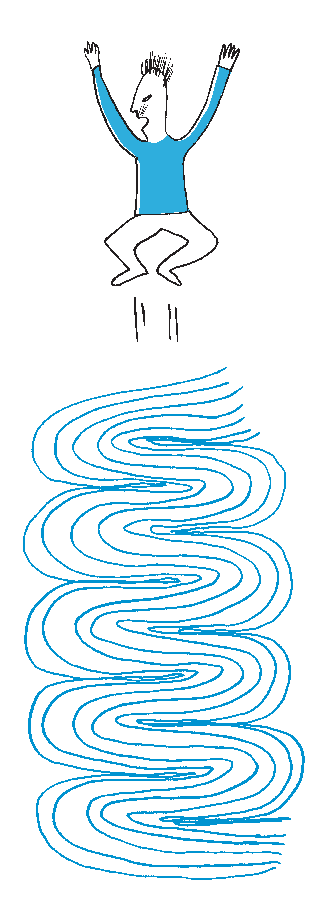
\includegraphics{art/202501_kol09}}
	

\eject